
写CMake时,有几个主要概念和语言特性需要知道。我们不会在这里详述语言的种种细节,若需要详细了解可以参考CMake的官方文档。下面的小节中,将简介主要概念和语言特性。后续章节将深入探讨其中细节。

完整文档地址\url{https://cmake.org/cmake/help/latest/manual/cmake-language.7.html}.

\subsubsubsection{1.6.1\hspace{0.2cm}CMake语言——一万英尺的全景}

CMake使用CMakeLists.txt文件的配置文件来确定构建规范。这些文件用脚本语言编写,通常也称为CMake。语言本身很简单,支持变量、字符串函数、宏、函数定义和导入其他CMake文件。

除了列表,不支持数据结构,如结构或类。但若操作得当,这种简单性使得CMake项目具有更好的可维护性。

语法基于关键字和以空格分隔的参数。例如,下面的指令会将相应的文件添加到库中:

\begin{lstlisting}[style=styleCMake]
target_sources(MyLibrary
                PUBLIC include/api.h
                PRIVATE src/internals.cpp src/foo.cpp)
\end{lstlisting}

PUBLIC和PRIVATE关键字表示文件链接到这个库时的可见性,并充当文件列表之间的分隔符。

此外,CMake语言支持“生成器表达式”,可以在生成构建系统时进行,通常用于为每个构建配置指定特殊信息。将在第3章进行详细介绍。

\hspace*{\fill} \\ %插入空行
\noindent
\textbf{工程}

CMake会将各种构建工件(如库、可执行文件、测试和文档)组织到项目中。虽然不同项目可以相互封装,但这里需要一个根项目。作为一个规则,每个CMakeLists.txt文件对应一个项目,这意味着每个项目必须在源目录中有一个单独的文件夹。

项目描述如下:

\begin{lstlisting}[style=styleCMake]
project(
  "chapter1"
  VERSION 1.0
  DESCRIPTION "A simple C++ project to demonstrate basic CMake
  usage" LANGUAGES CXX
)
\end{lstlisting}

正在解析的当前项目存储在PROJECT\_NAME变量中。根项目存储在CMAKE\_PROJECT\_NAME中,这对于确定一个项目是独立的还是封装在另一个项目中很有用。从3.21版本开始,还有一个PROJECT\_IS\_TOP\_LEVEL变量来直接确定当前项目是否是顶层项目。此外,使用<PROJECT-NAME>\_IS\_TOP\_LEVEL,可以检测特定的项目是否为顶级项目。

下面是关于项目的其他内置变量,它们可以在根项目的值前加上CMAKE\_前缀。若没有在\texttt{project()}指令中定义,则字符串为空:

\begin{itemize}
\item 
PROJECT\_DESCRIPTION: 项目的描述字符串

\item 
PROJECT\_HOMEPAGE\_URL: 项目的URL字符串

\item 
PROJECT\_VERSION: 这个项目的完整版本信息

\item 
PROJECT\_VERSION\_MAJOR: 版本字符串的第一个数字

\item 
PROJECT\_VERSION\_MINOR: 版本字符串的第二个数字

\item 
PROJECT\_VERSION\_PATCH: 版本字符串的第三个数字

\item 
PROJECT\_VERSION\_TWEAK: 版本字符串的第四个数字
\end{itemize}

每个项目都有一个源目录和二进制目录,它们可以相互封装。假设下面的例子中的每个CMakeFiles.txt文件都定义了一个项目:

\begin{tcblisting}{commandshell={}}
.
├── CMakeLists.txt #defines project("CMakeBestPractices"...)
├── chapter_1
│      ├── CMakeLists.txt # defines project("Chapter 1"...)
\end{tcblisting}

当解析根目录下的CMakeLists.txt文件时,PROJECT\_NAME和CMAKE\_PROJECT\_NAME都将是CMakeBestPractices。当解析chapter\_1/CMakeLists.txt时,PROJECT\_NAME变量将变为“chapter\_1”,但CMAKE\_PROJECT\_NAME还是CMakeBestPractices,并设置在根文件夹中。

尽管项目可以嵌套,但最好以独立的方式编写。虽然它们可能依赖于文件层次结构中较低的其他项目,但应该没有必要将一个项目作为另一个项目的子项目的必要。可以在同一个CMakeLists.txt文件中使用多个\texttt{project()},但并不推荐这样做,其会使项目混乱,难以维护。通常,最好为每个项目创建一个CMakeLists.txt文件,并用子文件夹组织结构。

本书的GitHub库,包含了本书中的例子,以分层的方式组织,其中每一章都是一个单独的项目,可能包含更多的项目,用于不同的部分和示例。

虽然每个示例都可以单独构建,但也可以从库的根目录构建整本书的所有示例。

\hspace*{\fill} \\ %插入空行
\noindent
\textbf{变量}

变量是CMake语言的核心部分。可以使用\texttt{set}指令设置变量,使用\texttt{unset}指令删除变量。变量名区分大小写。下面的例子展示了如何设置一个名为MYVAR的变量,并将其赋值为1234:

\begin{lstlisting}[style=styleCMake]
set(MYVAR "1234")
\end{lstlisting}

要删除MYVAR变量,可以使用\texttt{unset}:

\begin{lstlisting}[style=styleCMake]
unset(MYVAR)
\end{lstlisting}

一般的代码约定使用全大写命名变量。在内部,变量总是表示为字符串。

这里,可以用\$符号和花括号来访问变量的值:

\begin{lstlisting}[style=styleCMake]
message(STATUS "The content of MYVAR are ${MYVAR}")
\end{lstlisting}

变量的引用可以嵌套,并由内而外求值:

\begin{lstlisting}[style=styleCMake]
${outer_${inner_variable}_variable}
\end{lstlisting}

变量的作用域可以通过以下方式确定:

\begin{itemize}
\item 
函数作用域:在函数内部设置的变量只在函数内部可见。

\item 
目录作用域:源树中的每个子目录绑定变量,并包括来自父目录的任何变量。

\item 
持久缓存:缓存的变量可以是系统的,也可以是用户定义的。它们在多次运行中保持它们的值不变。
\end{itemize}

将PARENT\_SCOPE选项传递给\texttt{set()}会使变量在父作用域中可见。

CMake提供了各种预定义变量,通常以CMAKE\_为前缀。完整的列表地址\url{https://cmake.org/cmake/help/latest/manual/cmake-variables.7.html}。

\hspace*{\fill} \\ %插入空行
\noindent
\textbf{列表}

尽管CMake在内部将变量存储为字符串,但可以在CMake中使用分号分隔值来处理列表。列表可以通过传递多个未加引号的变量给\texttt{set()},或直接作为一个分号分隔的字符串来创建:

\begin{lstlisting}[style=styleCMake]
set(MYLIST abc def ghi)
set(MYLIST "abc;def;ghi")
\end{lstlisting}

使用\texttt{list}指令可以通过修改列表内容、重新排序或查找内容来操作列表。下面的代码将在MYLIST中查询abc值的索引,然后检索该值并将其存储在名为ABC的变量中:

\begin{lstlisting}[style=styleCMake]
list(FIND MYLIST abc ABC_INDEX)
list(GET MYLIST ${ABC_INDEX} ABC)
\end{lstlisting}

要向列表追加一个值,可以使用APPEND 关键字。这里,xyz值会添加到MYLIST中:

\begin{lstlisting}[style=styleCMake]
list(APPEND MYLIST "xyz")
\end{lstlisting}

\hspace*{\fill} \\ %插入空行
\noindent
\textbf{缓存变量和选项}

CMake caches some variables so that they run faster in subsequent builds. The variables are stored in CMakeCache.txt files. Usually, you don't have to edit them manually, but they are great for debugging builds that do not behave as expected. 

All the variables that are used to configure the build are cached. To cache a custom variable called ch1\_MYVAR with the foo value, you can use the set command, like this:

\begin{lstlisting}[style=styleCMake]
set(ch1_MYVAR foo CACHE STRING "Variable foo that configures bar")
\end{lstlisting}

Note that cached variables must have a type and a documentation string that provides
a quick summary of them.

Most of the cached variables that are automatically generated are marked as advanced, which means they are hidden from the user in cmake-gui and ccmake by default. To make them visible, they have to be toggled explicitly. If additional cache variables are generated by a CMakeLists.txt file, they can also be hidden by calling the mark\_as\_advanced(MYVAR) command:

\begin{center}
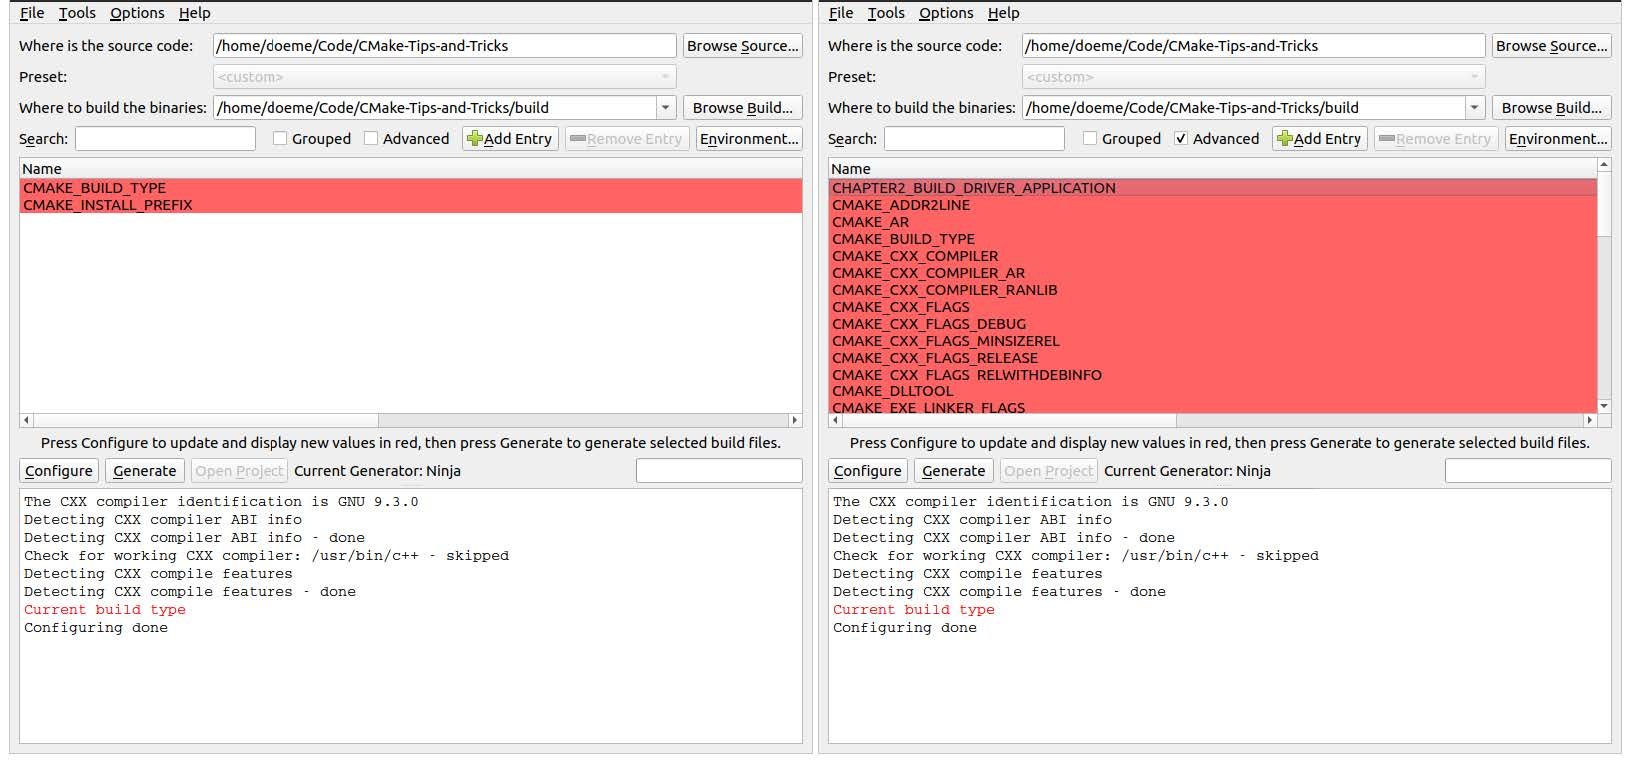
\includegraphics[width=0.8\textwidth]{content/1/chapter1/images/4.jpg}\\
Figure 1.4 – Left – cmake-gui does not show variables marked as advanced. Right – Marking the "Advanced" checkbox displays all the variables marked as advanced
\end{center}

As a rule of thumb, any option or variable that the user should change should be marked as advanced. This should happen rarely.

For simple Boolean cache variables, CMake also provides the option keyword. option
has a default value of OFF unless specified otherwise. They can also depend on each other via the CMakeDependentOption module:

\begin{lstlisting}[style=styleCMake]
option(CHAPTER1_PRINT_LANGUAGE_EXAMPLES "Print examples for 
	each language" OFF)
include(CMakeDependentOption)
cmake_dependent_option(CHAPTER1_PRINT_HELLO_WORLD "print a
	greeting from chapter1 " ON CHAPTER1_PRINT_LANGUAGE_EXAMPLES
		ON)
\end{lstlisting}

Options are often a convenient way to specify simple project configuration. They are cache variables of the bool type. If a variable with the same name as the option already exists, a call to option does nothing.

\hspace*{\fill} \\ %插入空行
\noindent
\textbf{属性}

Properties in CMake are values that are attached to a specific object or scope of CMake, such as a file, target, directory, or test case. Properties can be set or changed by using the set\_property function. To read the value of a property, you can use the get\_property function, which follows a similar pattern. By default, set\_property overwrites the values that are already stored inside a property. Values can be added to the current value by passing APPEND or APPEND\_STRING to set\_property.

The full signature is as follows:

\begin{lstlisting}[style=styleCMake]
set_property(<Scope> <EntityName>
			[APPEND] [APPEND_STRING]
			PROPERTY <propertyName> [<values>])
\end{lstlisting}

The scope specifier may have the following values:

\begin{itemize}
\item 
GLOBAL: Global properties that affect the whole build process.

\item 
DIRECTORY <dir>: Properties that are bound to the current directory or the directories specified in <dir>. These can also be set directly using the set\_directory\_properties command.

\item 
TARGET <targets>: Properties of specific targets. They can also be set using the set\_target\_properties function.

\item 
SOURCE <files>: Applies a property to a list of source files. They can also be set directly using set\_source\_files\_properties. Additionally, there are the SOURCE DIRECTORY and SOURCE TARGET\_DIRECTORY extended options:

\begin{itemize}
\item 
DIRECTORY <dirs>: This sets the property for the source files in the directory's scope. The directory must already be parsed by CMake by either being the current directory or by being added with add\_subdirectory.

\item 
TARGET\_DIRECTORY <targets>: This sets the property to the directory where the specified targets are created. Again, the targets must already exist at the point where the property is set.
\end{itemize}

\item 
INSTALL <files>: This sets the properties for installed files. These can be used to control the behavior of cpack.

\item 
TEST <tests>: This sets the properties for tests. They can also be set directly using set\_test\_properties.

\item 
CACHE <entry>: This sets the properties for cached variables. The most common ones include setting variables as advanced or adding documentation strings to them.
\end{itemize}

The full list of supported properties, sorted by their different entities, can be found at \url{https://cmake.org/cmake/help/latest/manual/cmakeproperties.7.html}.

It is good practice to use direct functions such as set\_target\_properties and set\_test\_properties when modifying properties instead of the more general set\_property command. Using explicit commands avoids making mistakes and confusion between the property names and is generally more readable. There's also the define\_property function, which creates a property without setting the value. We advise that you don't use this as properties should always have a sane default value.

\hspace*{\fill} \\ %插入空行
\noindent
\textbf{循环和条件}

Like any programming language, CMake supports conditional and loop blocks. Conditional blocks are in-between if(), elseif(), else(), and endif() statements. Conditions are expressed using various keywords.

Unary keywords are prefixed before the value, as shown here:

\begin{lstlisting}[style=styleCMake]
if(DEFINED MY_VAR)
\end{lstlisting}

The unary keywords to be used in conditions are as follows:

\begin{itemize}
\item 
COMMAND: True if the supplied value is a command

\item 
EXISTS: Checks whether a file or a path exists

\item 
DEFINED: True if the value is a defined variable
\end{itemize}

Additionally, there are unary filesystem conditions:

\begin{itemize}
\item 
EXISTS: True if the passed file or directory exits

\item 
IS\_DIRECTORY: Checks whether the supplied path is a directory

\item 
IS\_SYMLINK: True if the supplied path is a symbolic link

\item 
IS\_ABSOULTE: Checks whether a supplied path is an absolute path
\end{itemize}

Binary tests compare two values and are placed between the values to be compared, like this:

\begin{lstlisting}[style=styleCMake]
if(MYVAR STREQUAL "FOO")
\end{lstlisting}

The binary operators are as follows:

\begin{itemize}
\item 
LESS, GREATER, EQUAL, LESS\_EQUAL, and GREATER\_EQUAL: These compare numeric values.

\item 
STRLESS, STREQUAL, STRGREATER, STRLESS\_EQUAL, and STRGREATER\_EQUAL: These lexicographically compare strings.

\item 
VERSION\_LESS, VERSION\_EQUAL, VERSION\_GREATER, VERSION\_LESS\_EQUAL, and VERSION\_GREATER\_EQUAL: These compare version strings.

\item 
MATCHES: This compares against a regular expression.

\item 
IS\_NEWER\_THAN: Checks which of the two files that passed has been modified recently.

\item 
IS\_NEWER\_THAN: Unfortunately, this is not very precise because if both files have the same timestamp, it also returns true. There is also more confusion because if either of the files is missing, the result is also true.
\end{itemize}

Finally, there's the Boolean OR, AND, and NOT operators.

Loops are either achieved by while() and endwhile() or foreach() and endforeach(). Loops can be terminated using break(); continue() aborts the current iteration and starts the next one immediately.

while loops take the same conditions as an if statement. The following example loops as long as MYVAR is less than 5. Note that to increase the variable, we are using the math() function:

\begin{lstlisting}[style=styleCMake]
set(MYVAR 0)
while(MYVAR LESS "5")
	message(STATUS "Chapter1: MYVAR is '${MYVAR}'")
	math(EXPR MYVAR "${MYVAR}+1")
endwhile()
\end{lstlisting}

In addition to while loops, CMake also knows loops for iterating over lists or ranges:

\begin{lstlisting}[style=styleCMake]
foreach(ITEM IN LISTS MYLIST)
# do something with ${ITEM}
endforeach()
\end{lstlisting}

for loops over a specific range can be created by using the RANGE keyword:

\begin{lstlisting}[style=styleCMake]
foreach(ITEM RANGE 0 10)
# do something with ${ITEM}
endforeach()
\end{lstlisting}

Although the RANGE version of foreach() could work with only a stop variable, it is good practice to always specify both the start and end values.

\hspace*{\fill} \\ %插入空行
\noindent
\textbf{函数}

Functions are defined by function()/endfunction(). Functions open a new scope for variables, so all the variables that are defined inside are not accessible from the outside unless the PARENT\_SCOPE option is passed to set().

Functions are case-insensitive and are invoked by calling function, followed by parentheses:

\begin{lstlisting}[style=styleCMake]
function(foo ARG1)
# do something
endfunction()
# invoke foo with parameter bar
foo("bar")
\end{lstlisting}

Functions are a great way to make parts of your CMake reusable and often come in handy when you're working on larger projects.

\hspace*{\fill} \\ %插入空行
\noindent
\textbf{宏}

CMake macros are defined using the macro()/endmacro() commands. They are a
bit like functions, with the difference that in functions, the arguments are true variables, whereas in macros, they are string replacements. This means that all the arguments of a macro must be accessed using curly brackets.

Another difference is that by calling a function, control is transferred to the functions. Macros are executed as if the body of the macro had been pasted into the place of the calling state. This means that macros are not creating scopes regarding variables and control flow. Consequently, it is highly recommended to avoid calling return() in macros as this would stop the scope from executing where the macro is called.

\hspace*{\fill} \\ %插入空行
\noindent
\textbf{目标}

The build system of CMake is organized as a set of logical targets that correspond to an executable, library, or custom command or artifact, such as documentation or similar.

There are three major ways to create a target in CMake – add\_executable, add\_library, and add\_custom\_target. The first two are used to create executables and static or shared libraries, while the third can contain almost any custom command to be executed.

Targets can be made dependent on each other so that one target has to be built
before another.

It is good practice to work with targets instead of global variables when you're setting properties for build configurations or compiler options. Some of the target properties have visibility modifiers such as PRIVATE, PUBLIC, or INTERFACE to denote which requirements are transitive – that is, which properties have to be "inherited" by a dependent target.


\hspace*{\fill} \\ %插入空行
\noindent
\textbf{生成器表达式}

Generator expressions are small statements that are evaluated during the configuration phase of the build. Most functions allow generator expressions to be used, with a few exceptions. They take the form of \$<OPERATOR:VALUE>, where OPERATOR is applied or compared to VALUE. You can think of generator expressions as small inline if-statements.

In the following example, a generator expression is being used to enable the –Wall compiler flag for my\_target if the compiler is either GCC, Clang, or Apple Clang. Note that GCC is identified as COMPILER\_ID "GNU":

\begin{lstlisting}[style=styleCMake]
target_compile_options(my_target PRIVATE
	"$<$<CXX_COMPILER_ID:GNU,Clang,AppleClang>:-Wall>")
\end{lstlisting}

This example tells CMake to evaluate the CXX\_COMPILER\_ID variable to the commaseparated GNU, Clang, AppleClang list and that if it matches either, append the -Wall option to the target – that is, my\_target. Generator expressions come in very handy for writing platform- and compiler-independent CMake files. 

In addition to querying values, generator expressions can be used to transform strings and lists:

\begin{lstlisting}[style=styleCMake]
$<LOWER_CASE:CMake>
\end{lstlisting}

This will output cmake. 

You can learn more about generator expressions at \url{https://cmake.org/cmake/
help/latest/manual/cmake-generator-expressions.7.html}.

Since CMake supports a variety of build systems, compilers, and linkers, it is often used to build software for different platforms. In the next section, we will learn how CMake can be told which toolchain to use and how to configure the different build types, such as debug or release.

\hspace*{\fill} \\ %插入空行
\noindent
\textbf{CMake策略}

For the top-level CMakeLists.txt file, cmake\_minimum\_required must be called before any call to the project as it also sets which internal policies for CMake are used to build the project.

Policies are used to maintain backward compatibility across multiple CMake releases. They can be configured to use the OLD behavior, which means that cmake behaves backward compatible, or as NEW, which means the new policy is in effect. As each new version will introduce new rules and features, policies will be used to warn you of backwardcompatibility issues. Policies can be disabled or enabled using the cmake\_policy call.

In the following example, the CMP0121 policy has been set to a backward-compatible value. CMP0121 was introduced in CMake version 3.21 and checks whether index variables for the list() commands are in a valid format – that is, whether they are integers:

\begin{lstlisting}[style=styleCMake]
cmake_minimum_required(VERSION 3.21)
cmake_policy(SET CMP0121 OLD)

list(APPEND MYLIST "abc;def;ghi")
list(GET MYLIST "any" OUT_VAR)
\end{lstlisting}

By setting cmake\_policy(SET CMP0121 OLD), backward compatibility is enabled and the preceding code will not produce a warning, despite the access to MYLIST with the "any" index, which is not an integer.

Setting the policy to NEW will throw an error – [build] list index: any is not
a valid index – during the configuration step of CMake.

\hspace*{\fill} \\ %插入空行
\begin{tcolorbox}[colback=blue!5!white,colframe=blue!75!black,title=Avoid Setting Single Policies Except When You're Including Legacy Projects]
Generally, policies should be controlled by setting the cmake\_minimum\_required command and not by changing individual policies. The most common use case for changing single policies is when you're including legacy projects as subfolders.
\end{tcolorbox}

So far, we have covered the basic concepts behind the CMake language, which is used to configure build systems. CMake is used to generate build instructions for different kinds of builds and languages. In the next section, we will learn how to specify the compiler to use and how builds can be configured.












